\chapter*{Introduzione}
\markboth{INTRODUZIONE}{}
    Negli ultimi anni, l’Intelligenza Artificiale ha visto una crescita esponenziale in termini di popolarità, affidabilità e accessibilità economica, entrando a far parte della vita quotidiana in moltissimi settori. Le applicazioni basate su reti neurali sono ormai diffuse, facili da usare e alla portata di tutti, anche senza competenze specifiche, trovando spazio persino in contesti ludici. Un impatto significativo sicuramente lo si è riscontrato nel campo della sicurezza, dove l'IA viene progressivamente impiegata in ambiti che fino a poco tempo fa erano considerati esclusiva dell’intervento umano, grazie alla sua capacità di garantire prestazioni affidabili e costanti.
    Applicazioni come il controllo accessi, l’autenticazione sui dispositivi mobili, la videosorveglianza e il monitoraggio in spazi pubblici fanno largo uso di tecnologie biometriche, quali il riconoscimento delle impronte digitali, dell’iride e della voce, ognuna con specifici vantaggi in termini di precisione e contesto d’uso. Nello specifico, sono i sistemi di riconoscimento facciale spesso preferiti per la natura non invasiva, trainati dall’evoluzione dei sistemi di visione artificiale e delle reti neurali profonde.
    Tuttavia, come qualsiasi tecnologia, anche l’applicazione dell’Intelligenza Artificiale in contesti di sicurezza non è esente da potenziali vulnerabilità, che possono essere sfruttate da attaccanti per costruire exploit mirati a compromettere l’affidabilità dei sistemi. Ad esempio, è stato dimostrato che molti modelli di deep learning, pur essendo altamente accurati su immagini ``pulite'', possono essere ingannati da input artificialmente modificati. Tali input sono noti come \textit{adversarial examples} e consistono in perturbazioni impercettibili all’occhio umano, ma capaci di alterare drasticamente l’output del classificatore.
    Nel dominio della face recognition, questo tipo di attacco può avere implicazioni molto gravi: ad esempio, un volto opportunamente modellato, potrebbe essere riconosciuto come appartenente ad una determinata persona (\textit{error-specific}) oppure potrebbe essere etichettato erroneamente come appartenente ad un'identità qualsiasi, diversa da quella reale (\textit{error-generic}), consentendo così l’accesso a risorse riservate o l’elusione dei controlli. L’esistenza di queste vulnerabilità mina la fiducia nell’adozione su larga scala di questi sistemi, specialmente in ambiti ad alta criticità come aeroporti, strutture militari, banche e ambienti IoT.

    \begin{figure}[H]
        \centering
        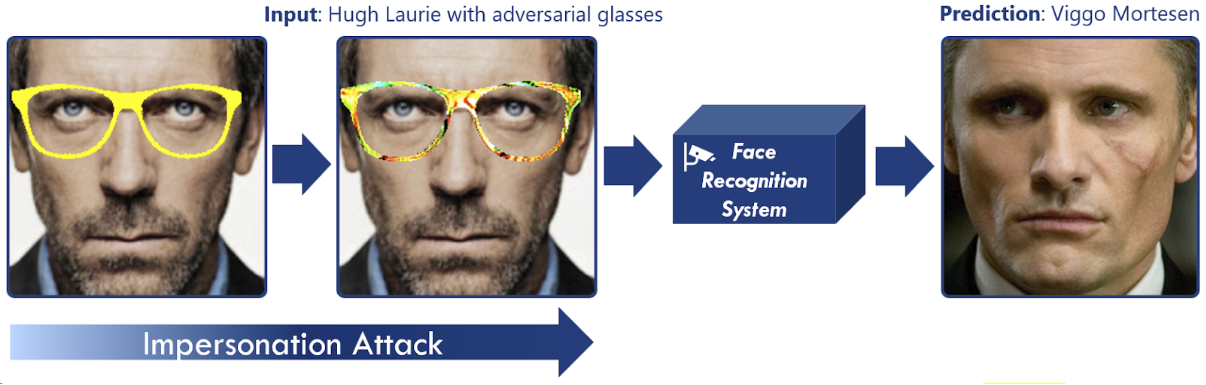
\includegraphics[width=0.95\textwidth]{images/impersonation_attack.png}
        \caption{Esempio di Face Recognition attack}
    \end{figure}

    \noindent Il presente progetto si propone di \textbf{valutare in modo sistematico la sicurezza di un sistema di face recognition} rispetto ad attacchi adversarial. A tal fine, ci siamo avvalsi di un sistema di riconoscimento facciale basato su un modello già esistente, del quale abbiamo preliminarmente valutato l’accuratezza su un test set appositamente costruito. Successivamente, il sistema è stato sottoposto a una serie di attacchi noti nella letteratura, sia di tipo error-generic che error-specific, al fine di analizzarne la risposta in presenza di input manipolati e valutarne l’eventuale degrado prestazionale, in particolare la difficoltà nel distinguere immagini autentiche da quelle contraffatte.
    Per approfondire il fenomeno della \textbf{trasferibilità} degli attacchi, gli stessi input avversari sono stati applicati anche a un secondo modello, basato su un’architettura differente, con l’obiettivo di indagare la capacità degli attacchi di conservare la propria efficacia anche su sistemi non direttamente conosciuti dall’attaccante, un aspetto cruciale nei contesti reali in cui spesso l’accesso al modello bersaglio non è esplicito.
    Infine, è stato implementato un meccanismo di difesa mirato a migliorare la robustezza del sistema originale nei confronti degli attacchi avversari, con l’intento di aumentarne l’affidabilità in scenari operativi.
    Il progetto si propone quindi come uno studio completo e sperimentale sulla robustezza dei moderni sistemi di face recognition, offrendo un contributo all’analisi delle loro vulnerabilità e alla progettazione di contromisure.
    Il lavoro è suddiviso nei seguenti capitoli:
        \begin{itemize}
            \item \textbf{Capitolo 1:} descrizione del dataset, criteri di selezione delle immagini, struttura del test set, pre-processing dei dati e analisi delle performance del modello;
            
            \item \textbf{Capitolo 2:} generazione di Adversarial Examples e analisi delle performance del modello;
            
            \item \textbf{Capitolo 3:} verifica della trasferibilità degli attacchi su un secondo modello;
            
            \item \textbf{Capitolo 4:} implementazione e valutazione di una strategia di difesa sul modello originale;
            
            \item \textbf{Capitolo 5:} conclusioni e riflessioni finali.
        \end{itemize}